%%%%%%%%%%%%%%%%%%%%%%%%%%%%%%%%%%%%%%%%%%%%%%%%%%%%%%%%%%%%%%%%%%%%%%%%%%%%%%%%%%%%
% Template for STAT 547C final project
% Author: Ben Bloem-Reddy <benbr@stat.ubc.ca>
% Date: Oct. 18, 2019
%%%%%%%%%%%%%%%%%%%%%%%%%%%%%%%%%%%%%%%%%%%%%%%%%%%%%%%%%%%%%%%%%%%%%%%%%%%%%%%%%%%%

% Note: You will get an empty bibliography warning when compiling until you include a citation.

\documentclass[10pt]{article}
% header.tex
% this is where you load pacakges, specify custom formats, etc.

\usepackage[left=1in,right=1in,top=0.75in,footskip=25pt]{geometry} 
% \usepackage{changepage}
\usepackage{amsmath,amsthm,amssymb,amsfonts}
\usepackage{mathtools}
% enumitem for custom lists
\usepackage{enumitem}
% Load dsfont this to get proper indicator function (bold 1) with \mathds{1}:
\usepackage{dsfont}
\usepackage{centernot}

\usepackage[usenames,dvipsnames]{xcolor}

% set up commenting code (I will use this during marking)
\definecolor{CommentColor}{rgb}{0,.50,.50}
\newcounter{margincounter}
\newcommand{\displaycounter}{{\arabic{margincounter}}}
\newcommand{\incdisplaycounter}{{\stepcounter{margincounter}\arabic{margincounter}}}
\newcommand{\COMMENT}[1]{\textcolor{CommentColor}{$\,^{(\incdisplaycounter)}$}\marginpar{\scriptsize\textcolor{CommentColor}{ {\tiny $(\displaycounter)$} #1}}}

\usepackage{appendix}

% set up graphics
\usepackage{graphicx}
\DeclareGraphicsExtensions{.pdf,.png,.jpg}
\graphicspath{ {fig/} }

\usepackage[sorting=nyt,backend=biber,bibstyle=alphabetic,citestyle=alphabetic,giveninits=true]{biblatex}

\usepackage{fancyhdr}
\pagestyle{fancy}
\setlength{\headheight}{40pt}

%%%%%%%%%%%%%%%%%%%%%%%%%%%%%%%%%%%%%%%%%%%%%%%%%%%%%%%%%%%%%%%%%%%%%%%%%%%%%%%%%%%%
% most other packages you might use should be loaded before hyperref
%%%%%%%%%%%%%%%%%%%%%%%%%%%%%%%%%%%%%%%%%%%%%%%%%%%%%%%%%%%%%%%%%%%%%%%%%%%%%%%%%%%%

% Set up hyperlinks:
\definecolor{RefColor}{rgb}{0,0,.65}
\usepackage[colorlinks,linkcolor=RefColor,citecolor=RefColor,urlcolor=RefColor]{hyperref}

\usepackage[capitalize]{cleveref}
\crefname{appsec}{Appendix}{Appendices} % you can tell cleveref what to call things
% defs.tex
% this is where you define custom notation, commands, etc.


%%
% full alphabets of different styles
%%

% bf series
\def\bfA{\mathbf{A}}
\def\bfB{\mathbf{B}}
\def\bfC{\mathbf{C}}
\def\bfD{\mathbf{D}}
\def\bfE{\mathbf{E}}
\def\bfF{\mathbf{F}}
\def\bfG{\mathbf{G}}
\def\bfH{\mathbf{H}}
\def\bfI{\mathbf{I}}
\def\bfJ{\mathbf{J}}
\def\bfK{\mathbf{K}}
\def\bfL{\mathbf{L}}
\def\bfM{\mathbf{M}}
\def\bfN{\mathbf{N}}
\def\bfO{\mathbf{O}}
\def\bfP{\mathbf{P}}
\def\bfQ{\mathbf{Q}}
\def\bfR{\mathbf{R}}
\def\bfS{\mathbf{S}}
\def\bfT{\mathbf{T}}
\def\bfU{\mathbf{U}}
\def\bfV{\mathbf{V}}
\def\bfW{\mathbf{W}}
\def\bfX{\mathbf{X}}
\def\bfY{\mathbf{Y}}
\def\bfZ{\mathbf{Z}}

% bb series
\def\bbA{\mathbb{A}}
\def\bbB{\mathbb{B}}
\def\bbC{\mathbb{C}}
\def\bbD{\mathbb{D}}
\def\bbE{\mathbb{E}}
\def\bbF{\mathbb{F}}
\def\bbG{\mathbb{G}}
\def\bbH{\mathbb{H}}
\def\bbI{\mathbb{I}}
\def\bbJ{\mathbb{J}}
\def\bbK{\mathbb{K}}
\def\bbL{\mathbb{L}}
\def\bbM{\mathbb{M}}
\def\bbN{\mathbb{N}}
\def\bbO{\mathbb{O}}
\def\bbP{\mathbb{P}}
\def\bbQ{\mathbb{Q}}
\def\bbR{\mathbb{R}}
\def\bbS{\mathbb{S}}
\def\bbT{\mathbb{T}}
\def\bbU{\mathbb{U}}
\def\bbV{\mathbb{V}}
\def\bbW{\mathbb{W}}
\def\bbX{\mathbb{X}}
\def\bbY{\mathbb{Y}}
\def\bbZ{\mathbb{Z}}

% cal series
\def\calA{\mathcal{A}}
\def\calB{\mathcal{B}}
\def\calC{\mathcal{C}}
\def\calD{\mathcal{D}}
\def\calE{\mathcal{E}}
\def\calF{\mathcal{F}}
\def\calG{\mathcal{G}}
\def\calH{\mathcal{H}}
\def\calI{\mathcal{I}}
\def\calJ{\mathcal{J}}
\def\calK{\mathcal{K}}
\def\calL{\mathcal{L}}
\def\calM{\mathcal{M}}
\def\calN{\mathcal{N}}
\def\calO{\mathcal{O}}
\def\calP{\mathcal{P}}
\def\calQ{\mathcal{Q}}
\def\calR{\mathcal{R}}
\def\calS{\mathcal{S}}
\def\calT{\mathcal{T}}
\def\calU{\mathcal{U}}
\def\calV{\mathcal{V}}
\def\calW{\mathcal{W}}
\def\calX{\mathcal{X}}
\def\calY{\mathcal{Y}}
\def\calZ{\mathcal{Z}}


%%%%%%%%%%%%%%%%%%%%%%%%%%%%%%%%%%%%%%%%%%%%%%%%%%%%%%%%%%
% text short-cuts
\def\iid{i.i.d.\ } %i.i.d.
\def\ie{i.e.\ }
\def\eg{e.g.\ }
\def\Polya{P\'{o}lya\ }
%%%%%%%%%%%%%%%%%%%%%%%%%%%%%%%%%%%%%%%%%%%%%%%%%%%%%%%%%%

%%%%%%%%%%%%%%%%%%%%%%%%%%%%%%%%%%%%%%%%%%%%%%%%%%%%%%%%%%
% quasi-universal probabilistic and mathematical notation
% my preferences (modulo publication conventions, and clashes like random vectors):
%   vectors: bold, lowercase
%   matrices: bold, uppercase
%   operators: blackboard (e.g., \mathbb{E}), uppercase
%   sets, spaces: calligraphic, uppercase
%   random variables: normal font, uppercase
%   deterministic quantities: normal font, lowercase
%%%%%%%%%%%%%%%%%%%%%%%%%%%%%%%%%%%%%%%%%%%%%%%%%%%%%%%%%%

% operators
\def\P{\bbP} %fundamental probability
\def\E{\bbE} %expectation
% conditional expectation
\DeclarePairedDelimiterX\bigCond[2]{[}{]}{#1 \;\delimsize\vert\; #2}
\newcommand{\conditional}[3][]{\bbE_{#1}\bigCond*{#2}{#3}}
\def\Law{\mathcal{L}} %law; this is by convention in the literature
\def\indicator{\mathds{1}} % indicator function
\def\Var{\mathrm{Var}}
\def\Cov{\mathrm{Cov}}

% sets and groups
\def\borel{\calB} %Borel sets
\def\sigAlg{\calA} %sigma-algebra
\def\filtration{\calF} %filtration
\def\grp{\calG} %group

% binary relations
\def\condind{{\perp\!\!\!\perp}} %independence/conditional independence
\def\equdist{\stackrel{\text{\rm\tiny d}}{=}} %equal in distribution
\def\equas{\stackrel{\text{\rm\tiny a.s.}}{=}} %euqal amost surely
\def\simiid{\sim_{\mbox{\tiny iid}}} %sampled i.i.d

% common vectors and matrices
\def\onevec{\mathbf{1}}
\def\iden{\mathbf{I}} % identity matrix
\def\supp{\text{\rm supp}}

% misc
% floor and ceiling
\DeclarePairedDelimiter{\ceilpair}{\lceil}{\rceil}
\DeclarePairedDelimiter{\floor}{\lfloor}{\rfloor}
\newcommand{\argdot}{{\,\vcenter{\hbox{\tiny$\bullet$}}\,}} %generic argument dot
%%%%%%%%%%%%%%%%%%%%%%%%%%%%%%%%%%%%%%%%%%%%%%%%%%%%%%%%%%

%%%%%%%%%%%%%%%%%%%%%%%%%%%%%%%%%%%%%%%%%%%%%%%%%%%%%%%%%%
%% some distributions
% continuous
\def\UnifDist{\text{\rm Unif}}
\def\BetaDist{\text{\rm Beta}}
\def\ExpDist{\text{\rm Exp}}
\def\GammaDist{\text{\rm Gamma}}
% \def\GenGammaDist{\text{\rm GGa}} %Generalized Gamma
\def\GP{\mathrm{GP}}

% discrete
\def\BernDist{\text{\rm Bernoulli}}
\def\BinomDist{\text{\rm Binomial}}
\def\PoissonPlus{\text{\rm Poisson}_{+}}
\def\PoissonDist{\text{\rm Poisson}}
\def\NBPlus{\text{\rm NB}_{+}}
\def\NBDist{\text{\rm NB}}
\def\GeomDist{\text{\rm Geom}}
% \def\CRP{\text{\rm CRP}}
% \def\EGP{\text{\rm EGP}}
% \def\MittagLeffler{\text{\rm ML}}
%%%%%%%%%%%%%%%%%%%%%%%%%%%%%%%%%%%%%%%%%%%%%%%%%%%%%%%%%%

%%%%%%%%%%%%%%%%%%%%%%%%%%%%%%%%%%%%%%%%%%%%%%%%%%%%%%%%%%
% Project-specific notation should go here
% (Because it's at the end of the file, it can overwrite anything that came before.)

%e.g.,
\def\Laplacian{\calL}
\def\P{\calP}

% combinatorial objects
\def\perm{\sigma} %fixed permutation
\def\Perm{\Sigma} %random permutation
\def\part{\pi} %fixed partition
\def\Part{\Pi} %random partition


%%%%%%%%%%%%%%%%%%%%%%%%%%%%%%%%%%%%%%%%%%%%%%%%%%%%%%%%%%

%%%%%%%%%%%%%%%%%%%%%%%%%%%%%%%%%%%%%%%%%%%%%%%%%%%%%%%%%%%%%%%%%%%%%%%%%%%%%%%%%

% your title/author/date information go here
\title{Exchangeability in Dependence Modelling} % replace with your title
\author{Gian Carlo Di-Luvi 
\\
{\normalsize Department of Statistics, University of British Columbia}} % replace with your name
\date{\normalsize December 10, 2019} % replace with your submission date

\bibliography{../../ref/STAT_547C.bib} % add the title of your bibliography file

% start of document
\begin{document}

\maketitle
\thispagestyle{empty}

\vskip 0.5cm

\begin{abstract}
\noindent Exchangeability is a fundamental concept in probability theory which has profound theoretical implications, amongst them de Finetti's representation theorem. Essentially, any exchangeable sequence---one that is distribution-invariant under finite permutations---can be represented as conditionally independent given a unique measure. However, in situations in which the process of interest depends on a sequence of covariates, exchangeability is seldom satisfied. Multiple extended notions of exchangeability have been proposed to overcome this, with some of them even having de Finetti-like representation theorems. We study three specific notions of exchangeability that play a central role in dependence modelling: partial, local, and regression exchangeability. We argue that there is a trade-off between how adequate each notion is and how powerful it can be in terms of theoretical implications. Furthermore, we do an in-depth study of these concepts in the context of Gaussian process regression, finding that most of the expanded notions of exchangeability are satisfied by it. This means that representation theorems for Gaussian processes do exist, and simple modifications of the arguments we present generalize this for other models for statistical dependence. Whether a Gaussian process has noisy observations or not also plays a central role in determining its exchangeability, which hints at the stark difference of models with and without replicates. Lastly, we conjecture a representation theorem for regression exchangeability, which to the best of our knowledge does not yet exist. This would make this relatively new notion a powerful theoretical tool for regression analysis.
\end{abstract}

\textbf{Keywords:} exchangeability; representation theorem; dependence modelling; Gaussian process regression.




% background section
\cleardoublepage
\setcounter{page}{1}
% !TEX root = ../main.tex

% Background section

\section{Introduction}


A sequence of random variables taking values in a standard measurable space $(\calX, \calB)$ is said to be exchangeable if the distribution of any finite subsequence of it is invariant under permutations. Formally:

\begin{definition}[Exchangeability] \label{def:exchangeability}
	The random variables $X_1, ..., X_n$ are said to be finitely exchangeable if
	\begin{equation*}
		(X_1, ..., X_n) \equdist (X_{\pi(1)}, ..., X_{\pi(n)})
	\end{equation*}
	for any permutation $\pi$ of $\bbN_n :=\{1, ..., n \}$.\footnote{For the sake of completeness, a permutation $\pi$ of a set $\calH$ is simply a bijection in $\calH$.} A countable sequence $(X_n)_{n=1}^{\infty}$ of random variables is said to be exchangeable if every finite subsequence of it is finitely exchangeable.
\end{definition}

%The notion of exchangeability captures a sense of homogeneity in the population, but it is a weaker assumption than independence and identical distribution, as we show in the following example.

%\begin{mdframed}[backgroundcolor=mygray] 
%	\begin{example} \label{ex:iid_exch}
%		Let $X_1, X_2, ...$ be i.i.d. random variables with common distribution $\mu$. For $n \in \bbN$ consider (without loss of generality) the subsequence $X = (X_1, ..., X_n)$. Then the joint distribution $\mu_n$ of $X$ is, due to independence, the $n$-product of $\mu$: $\mu_n = \mu \times \mu \times \cdots \times \mu$. For any permutation $\pi$ of $\bbN_n$ it is possible to trivially rearrange the products, and so clearly $X \equdist (X_{\pi(1)}, ..., X_{\pi(n)})$. Hence, any i.i.d. sequence is exchangeable.
%	\end{example}
%\end{mdframed}



This seemingly innocent definition captures a sense of homogeneity in the process and has a very profound consequence---namely, de Finetti's representation theorem, which has been proved in increasing generality \cite{deFinetti:1930:RepTheorem, HewittSavage:1955:rep_theorem, DiaconisFreedman:1978:Generalizations} and we now state for reference.

\begin{theorem}[de Finneti] \label{thm:definetti}
	$(X_n)_{n=1}^{\infty}$ is an exchangeable sequence of random variables if and only if there exists a unique probability measure $\mu$ on $\calP$---the set of all probability measures on $(\calX, \calB)$---such that
	\begin{equation} \label{eq:definetti_thm}
		\bbP \{ X_1 \in A_1, ..., X_n \in A_n \} = \int_{\calP}  \prod_{i=1}^n F(A_i) \, \mu(dF)
	\end{equation} 
	for every $n \in \bbN$ and $A_1, ..., A_n \in \calB$.\footnote{Observe that the integral in Equation (\ref{eq:definetti_thm}) is over a set of functions---namely, the set of probability measures on $(\calX, \calB)$.}
\end{theorem}




Technicalities aside, Theorem \ref{thm:definetti} intuitively tells us that, conditional on an unknown distribution $F$---which is always guaranteed to exist---any subsequence of an exchangeable process can be thought of as a random sample with common distribution $F$. This distribution plays the role of an infinite-dimensional parameter \cite[][Ch.~4.3]{BernardoSmith:1994:BayesianTheory}. Furthermore, $F$ has a unique prior distribution $\mu$, which justifies the use of a Bayesian approach in settings with exchangeable data.


\begin{mdframed}[backgroundcolor=mygray] 
	\begin{example} \label{ex:binary_definetti}
		Let $X = X_1, X_2, ...$ be an exchangeable sequence of binary random variables, that is, $\calX = \{0, 1\}$. In this case \cite[see][p.111]{Diaconis:1988:PartialExchang}, de Finetti's theorem asserts the existence of a unique measure $\mu$ such that, for every $n \in \bbN$ and $x_1, ..., x_n \in \calX$,
		\begin{equation*}
			\bbP \{ X_1 = x_1, ..., X_n = x_n \} = \int \mu(dp) \, p^s (1-p)^{n-s},
		\end{equation*}
		where $s = \sum_{i=1}^n x_i$ is the number of 1's in the sequence $x_1, ..., x_n$. In other words, there exists a random variable $p$ in the unit interval with distribution $\mu$ such that, given $p$, $X_1, ..., X_n$ are i.i.d. Bernoulli random variables with parameter $p$.
	\end{example}
\end{mdframed}








In many practical situations, however, one is interested in studying not a single isolated sequence of random variables, but its relationship---and dependence---with a sequence of covariates. It may at first sight seem that exchangeability has no role to play in statistical models for dependence, but we argue that this is not so. Multiple generalizations of the notion of exchangeability, some of which are satisfied in this dependence modeling setting, have been proposed since at least 1938 \cite{deFinetti:1938:partial_exch}. For example, \cite{Aldous:2010, Orbanz:Roy:2015} expand exchangeability for a wide variety of random arrays and graphs; \cite{Bernardo:1996:Exch, CamerlenghiEtAl:2019:partial_exchang_hierarchical} discuss it in a hierarchical modeling setting; and \cite{Diaconis:1988:PartialExchang} reviews its uses in Markov Chains. Furthermore, de Finetti-like representation theorems exist for some of these notions of exchangeability. 
\\


In this work we are interested in studying the role that exchangeability can play in dependence modelling, that is, when the distribution of the variables of interest depends on a set of covariates. Special emphasis is given to Gaussian process regression models \cite{RasmussenWilliams:2006}, an area that has seen a surge in popularity over the last years, especially in the modelling of complex phenomena, statistical emulation, and Bayesian optimization.
\\


For this purpose we first define, in Section \ref{section:exchangeability}, three extensions of the notion of exchangeability that are of use in dependence modelling: partial exchangeability \cite{deFinetti:1938:partial_exch}, local exchangeability \cite{CampbellEtAl:2019:LocalExch}, and regression exchangeability \cite{McCullagh:2005:ExchAndReg}. Their benefits and disadvantages are discussed and de Finetti-like representation theorems are stated whenever available. In Section \ref{section:GPs} we then give a brief overview of Gaussian process regression, and study it in the context of exchangeability. We conclude in Section \ref{section:discussion} with a brief discussion and possible future research directions.





% ...

\vskip 2cm

% add your main body sections here

% exchangeability section
% !TEX root = ../main.tex

% Exchangeability section

\section{Beyond exchangeability} \label{section:exchangeability}




There are very general settings where even exchangeability is too strong an assumption. Consider the case of a sequence $(X_n)$ of random variables endowed with covariates $(t_n)$, and such that the distribution of each $X_i$ depends on $t_i$. It is clear that $(X_n)$ is not an exchangeable sequence, and so de Finetti's representation theorem cannot be immediatly used. Some more general notions of exchangeability to overcome this difficulty have been proposed.



\subsection{Partial exchangeability}


de Finetti \cite{deFinetti:1938:partial_exch} introduced the concept of \textit{partial exchangeability} precisely for settings in which the variables of interest have covariates. The idea, which we formalize below, is to require exchangeability only for variables with the same covariate values.

\begin{definition}[Partial exchangeability] \label{def:partial_exchangeability}
	Let $X = (X_n)_{n=1}^{\infty}$ be a sequence of random variables, each one of them endowed with a covariate $t_n \in \calT$. For every $t \in \calT$ define the $t$-class $X_t$ to be the subsequence of $X$ such that all the covariates of $X_t$ are $t$, that is,
	\begin{equation*}
		X_t = \{ X_n \; : \; t_n = t \}.
	\end{equation*}
	Then the sequence $X$ is said to be partially exchangeable if all of its classes are exchangeable.
\end{definition}

A partially exchangeable sequence can be naturally grouped in an array-like fashion according to the different values that the covariates take. Specifically, suppose that $\calT = \{t_1, ..., t_d \}$, so that there are $d$ classes. Then the sequence $\left\{ (X_{t_i, \, n})_{n=1}^{\infty} \, : \, i=1, ..., d \right\}$ is a partially exchangeable sequence if $(X_{t_i, \, n})_{n=1}^{\infty}$ is exchangeable for each $i=1, ...d$. \\

Under the assumption that every class is countably infinite, a representation theorem analogous to \ref{thm:definetti} exists. Before giving a more formal statement, we showcase an example.


\begin{mdframed}[backgroundcolor=mygray] 
	\begin{example} 
		Consider an experiment in which two types of binary observations, $(X_{0, \, n})_{n=1}^{\infty}$ and $(X_{1, \, n})_{n=1}^{\infty}$, are under study. For example, $X_{0, \, i}$ could measure if a male patient recovered (1) or not (0) after taking a certain medication, while $X_{1, \, i}$ would measure the same outcome but for a female patient. In this case the covariate $t_n$ is also binary, and only indicates whether the patient is male (0) or female (1). Hence, there are two classes: $X_0$ and $X_1$, which correspond to male and female patients, respectively. \\
		
		If it is deemed that the value of the covariate does not affect the outcome of the variables, then exchangeability of the sequence $X = (X_0, X_1)$ might be a feasible assumption. If this is not so, it might still be feasible to assume exchangeability within male patients and whithin female patients. In that case, $X$ would be partially exchangeable. \\
		
		Furthermore, for such a partially exchangeable process there exists a measure $\mu$ such that, for every $l, r \in \bbN$,
				\begin{equation*}
			\bbP \{ X_{0, \, 1} = m_1, ..., X_{0, \, l} = m_l, X_{1, \, 1} = f_1, ..., X_{1, \, r} = f_r \} = \iint  \mu(dp_0, dp_1) \, p_0^{s_0} (1-p_0)^{l-s_0} \, p_1^{s_1} (1-p_1)^{r-s_1},
		\end{equation*}
		where $s_0 = \sum_{i=1}^l m_i$ and $s_1 = \sum_{i=1}^r f_i$ are the number of 1's in the male and female groups, respectively \cite[][p.~112-113]{Diaconis:1988:PartialExchang}.
	\end{example}
\end{mdframed}

We now state the representation theorem for general partially exchangeable sequences. (Adapted from \cite[][p.~69]{CamerlenghiEtAl:2019:partial_exchang_hierarchical}.)


\begin{theorem} \label{thm:definetti_partial}
	$\left\{ (X_{t_i, \, n})_{n=1}^{\infty} \, : \, i=1, ..., d \right\}$ is a partially exchangeable sequence if and only if there exists a unique probability measure $\mu$ on $\calP^d$ such that, for all $n_1, ..., n_d \in \bbN$ and $A_1, ..., A_d \in \calB^{n_i}$,
	\begin{equation} \label{eq:definetti_partial_thm}
		\bbP \left\{ (X_{t_i, \, k})_{k=1}^{n_i} \in A_i \, : \, i=1, ..., d  \right\} = \int_{\calP^d}  \prod_{i=1}^d F_i(A_i) \, \mu(dF_1, ..., dF_d).
	\end{equation}
\end{theorem}



As per Theorem \ref{thm:definetti}, every distribution $F_i$ in Equation (\ref{eq:definetti_partial_thm}) is itself a product measure on $\calX^{n_i}$. \\


Finally, observe that partial exchangeability requires access to so-called replicates: at each value of the covariate, an infinite number of response variables can be, at least in theory, obtained (or considered). Although this is true for cases as the one in Example \ref{ex:binary_definetti}, it does not always hold.



\subsection{Local exchangeability}


Campbell et al. \cite{CampbellEtAl:2019:LocalExch} propose the notion of \textit{local exchangeability} for data with covariates. Both exchangeability and partial exchangeability require some sort of strict invariance under permutations. In this case this is relaxed to allow for some distributional variation under permutations, so long as this variation is bounded and proportional to how close the corresponding covariates are. Interestingly, a representation theorem can still be obtained in such a scenario. Before formalizing these ideas, we define a way to measure variation between distributions.


\begin{definition}[Total variation distance]
	Let $X, Y$ be random variables taking values in a measurable space $(E, \calE)$. Then the total variation between $X$ and $Y$ is
	\begin{equation*}
		d_{\mathrm{TV}} (X, Y) = \sup_{A \in \calE} \left| \bbP \{ X \in A \} - \bbP \{Y \in A \} \right|.
	\end{equation*}
\end{definition}


\begin{definition}[Local exchangeability] \label{def:local_exchangeability}
	Let $X = (X_t)_{t \in \calT}$ be a sequence of random variables with covariate space $\calT$ and $d: \calT \times \calT \to \bbR_{+}$ a pseudometric (distances between different points need not be positive). The process $X$ is said to be $f$-locally exchangeable if there exists a function $f: \bbR_{+} \to \bbR_{+}$ continuous at zero and with $f(0) = 0$ such that, for every finite subset $T \subset \calT$ and permutation $\pi$ of $T$,
	\begin{equation} \label{eq:local_exch}
		d_{\mathrm{TV}} (X_T, X_{\pi T}) \leq \sum_{t \in T} f(d(t, \pi(t))).
	\end{equation}
\end{definition}


For a very rich discussion of this idea see \cite{CampbellEtAl:2019:LocalExch}, where the authors discuss e.g. the usage of the total variation distance instead of other divergence measures, and provide some examples of locally-exchangeable processes from the Bayesian nonparametrics literature. \\



We now state the main result for local exchangeability. The idea behind it is that, so long as the covariate space $\calT$ is ``nice,'' a de Finetti-like representation of $f$-locally exchangeable sequences exists in terms of a stochastic process $G$, conditional on which the sequence exhibits independence (Equation \ref{eq:local_exch_1}). Furthermore, the function $f$ controls the ``smoothness'' behaviour of $G$ (Equation \ref{eq:local_exch_2}). 

\begin{theorem}[Campbell et al. (2019)] \label{thm:de_finetti_local}
	Let $X = (X_t)_{t \in \calT}$ be a stochastic process on a separable space $\calT$, which furthermore has no isolated points under the pseudometric $d$. Then $X$ is $f$-locally exchangeable if and only if there exists a random measure-valued stochastic process $G = (G_t)_{t \in \calT}$ such that, for any finite subset of covariates $T \in \calT$ and permutation $\pi$ of $T$,
	\begin{equation} \label{eq:local_exch_1}
		\bbP \{ X_T \in \cdot \, | \, G \} \overset{\mathrm{a.s.}}{=} \prod_{t \in \calT} G_t := G_T
	\end{equation}
	and
	\begin{equation} \label{eq:local_exch_2}
		\sup_{A} \bbE \left| G_T(A) - G_{\pi T} (A) \right| \leq \sum_{t \in \calT} f(d(t, \pi(t))).
	\end{equation}
	Furthermore, $G$ is unique up to modification, that is, if $G'$ also satisfies Equations (\ref{eq:local_exch_1}) and (\ref{eq:local_exch_2}) then $\bbP \left\{ G_t = G_t^{'} \right\} = 1$ for all $t \in \calT$.
\end{theorem}


Local exchangeability manages to relax the requirements of exchangeability and partial exchangeability while still preserving a representation result. However, in doing so, the cost it pays is an increased complexity in the calculations involved. Where most processes can be easily determined to be either (partially) exchangeable or not---sometimes even by construction---actually proving a sequence to be locally exchangeable is not an easy feat. Proposition \ref{prop:sufficient_local_exchangeability} provides sufficient conditions which make this task easier, but only marginally so. 



\subsection{Regression exchangeability}



McCullagh \cite{McCullagh:2005:ExchAndReg} proposed yet another notion of exchangeability. Unlike the previous ideas so far discussed, McCullagh aims not for generality but for a definition that works well specifically in a regression setting, appealing to the idea that exchangeability should capture a sense of homogeneity.

\begin{definition}[Regression exchangeability]	\label{def:regression_exchangeability}
	Let $X = (X_n)_{n=1}^{\infty}$ be a sequence of random variables, each one of them endowed with a covariate $t_n \in \calT$. The sequence $X$ is said to be regression exchangeable (modulo $T = (t_n)$) if given two arbitrary subsets $T_1, T_2 \subset T$ of the covariate space the following two conditions hold:
	\begin{enumerate}
		\item If $T_1 \subset T_2$ then the distribution of $X_{T_1}$ must be the marginal distribution of $X_{T_2}$ under co-ordinate deletion. \label{cond:reg_exch_1}
		\item If $T_1 = T_2$ then $X_{T_1} \equdist X_{T_2}$. \label{cond:reg_exch_2}
	\end{enumerate}
\end{definition}


Condition \ref{cond:reg_exch_1} in Definition \ref{def:regression_exchangeability} simply ensures compatibility with respect to subsampling from $X$, and in the context of Gaussian process regression it is known as the \textit{marginalization} property \cite[][p.~13]{RasmussenWilliams:2006}. Condition \ref{cond:reg_exch_2} may seem trivial, but observe that $X_{T_1}$ and $X_{T_2}$ may very well be different. However, so long as their covariates are the same, any distinction between the actual values within $X_{T_1}$ and $X_{T_2}$ has no effect on their distribution. We showcase this with an example.



\begin{mdframed}[backgroundcolor=mygray] 
	\begin{example} \label{ex:reg_exch_1}
		Let $X = X_1, X_2, ...$ be independent random variables such that $X_i \sim \calN (\eta + \tau_{t_i}, 1)$, where $T = (t_n)_{n=1}^{\infty} = (1, 2, 3, 1, 2, 3, ...)$. $X$, which can be thought of as the response of an experiment with one factor and three levels, has independent components, but is nonetheless not exchangeable. However, $X$ is clearly regression exchangeable (modulo $T$): given $T_1, T_2 \subset T$, $X_{T_1}$ is the sample of such an experiment and follows a multivariate Normal distribution with covariance matrix $\sigma^2 I_{|T_1|}$ and mean vector $(\eta + \tau_{t_i})_{t_i \in T_1}$, and similarly with $T_2$. Clearly if $T_1 \subset T_2$ then the distribution of $T_1$ is obtained by ``removing'' the covariates in $T_2 \setminus T_1$. Furhermore, if $T_1 = T_2$ then (even if the actual $X_i$'s selected are different) $X_{T_1} \equdist X_{T_2}$.
	\end{example}
\end{mdframed}


Example \ref{ex:reg_exch_1} works well due to the availability of replicates. However, unlike partial exchangeability (Example \ref{ex:binary_definetti}), a process may not have replicates at all and still be regression exchangeable, whereas it would not be partially so. However, it is worth noting that Condition \ref{cond:reg_exch_2} in Definition \ref{def:regression_exchangeability} does reduce to a triviality in such a setting: the only way $T_1 = T_2$ would be if $X_{T_1} = X_{T_2}$ exactly. \\

To the best of our knowledge, there is no de Finetti-like representation theorem available for regression exchangeability.




% ...

\vskip 2cm


% GPs section
% !TEX root = ../main.tex

% Gaussian process regression section

\section{Gaussian process regression} \label{section:GPs}


Consider a sequence of random variables $X = (X_t)_{t \in \calT}$ endowed with covariates in the space $\calT$ and a finite subset $X_T$, $T \subset \calT$ of them. Suppose we are interested in studying $X_{t^{*}}$ for $t^{*} \notin T$, given $X_T$. A natural estimator would be $\bbE [X_{t^{*}} \, | \, \sigma X_T ]$, which of course depends on the distributional and dependence structures of the process $X$. If $X$ is a Gaussian process, which we define below, this expression can be easily computed and the methodology just discusses is called Gaussian process regression. This method has gained popularity in the last years as a reliable way of modelling complex phenomena, such as computer experiments \cite{SacksEtAl:1989:CompExp} and disease spreading \cite{PokharelDeardon:2016:GPInfectDisease}, and for doing Bayesian optimization \cite{Frazier:2018:BayesOptTutorial} and statistical emulation \cite{WoodsEtAl:2017:ACEAlgorithm}.



\begin{definition}[Gaussian process] \label{def:GP}
	A stochastic process $X = (X_t)_{t \in \calT}$ is said to be a Gaussian process (GP) if, for any finite subset $T \subset \calT$, $X_T$ follows a Normal distribution. 
\end{definition}


\textbf{Remark.} A Gaussian process is entirely determined by its mean $m$ and covariance $\kappa$ functions. Formally, $m: t \mapsto \bbE[X_t]$ and $\kappa: (t, t') \mapsto \Cov(X_t, X_{t'})$ and we write $X \sim \GP (m, \kappa)$. Commonly, $m$ is assumed to be zero and $\kappa$ is chosen from some parametric family of functions, many of which have been thoroughly studied in the literature \cite[see][Ch.~4]{RasmussenWilliams:2006}. Unless otherwise stated, we use a standard squared exponential covariance function,
\begin{equation} \label{eq:sq_exp_cov}
	\kappa(t, t') = \kappa(|t-t'|) = \mathrm{exp} \left\{ -\frac{1}{2} |t-t'|^2 \right\}.
\end{equation}



In practice, GP regression commonly arises when studying functions which are computationally expensive to evaluate. The general idea is to assume that the function of interest $f$ is a GP and use a sample of values of $f$ to estimate the function in unobserved values of the domain. Formally, consider a function $f: \calT \to \bbR$ and denote $X_t := f(t)$ for all $t \in \calT$. We assume that $X = (X_t) \sim \GP (m, \kappa)$. Usually, $\calT$ will be a subset of $\bbR^n$, $m = 0$ and we will have access to observations $(X_t, t)_{t \in T}$, where $T$ is a finite subset of $\calT$. If this is the case,
\begin{equation} \label{eq:GP_noise_free}
	X_T \equdist \calN (0, K(T, T)),
\end{equation}
where $K$ is a $|T| \times |T|$ matrix with entries $K_{ij} = \kappa(t_i, t_j)$. If we want to predict the value of the function $f(t^{*})$, we again use the fact that
\begin{equation*}
	\begin{pmatrix} X_T \\ X_{t^{*}} \end{pmatrix} \equdist \calN \left( 0, \begin{pmatrix} K(T, T) & K(T, t^{*}) \\ K(t^{*}, T) & \kappa(t^{*}, t^{*}) \end{pmatrix} \right),
\end{equation*}
from where, using basic properties of the Normal distribution,
\begin{equation} \label{eq:GPupdate}
	\bbP [X_{t^{*}} \,| \, \sigma X_T ] \equdist \calN \left( K(t^{*}, T) K(T, T)^{-1} X_T, \, \kappa(t^{*}, t^{*}) K(t^{*}, T) K(T, T)^{-1} K(T, t^{*})  \right).
\end{equation}
Equation (\ref{eq:GPupdate}) gives us not only the conditional expectation discussed earlier, but the whole conditional distribution: $\bbP [X_{t^{*}} \,| \, \sigma X_T ]$ is a Normally-distributed random variable. Commonly, the conditional mean in Equation (\ref{eq:GPupdate}) is used as a point estimate $\tilde{f}$ of $f$:
\begin{equation} \label{eq:GP_posteriormean}
	\tilde{f} (t^{*}) = \bbE [ X_{t^{*}} \, | \, \sigma X_T ] = K(t^{*}, T) K(T, T)^{-1} X_T.
\end{equation}
The estimated variance can be used to e.g. compute (conditional) confidence bands. Also, observe that we could have well chosen $t^{*}$ to have more than one component if we were interested in values of $f$ only at specific points in the covariate space. The advantage of Equation (\ref{eq:GP_posteriormean}) is that it provides point estimates for \textit{any} point in $\calT$. Figure \ref{fig:GP1} showcases this process. \\




\begin{figure}[h]
	\centering
	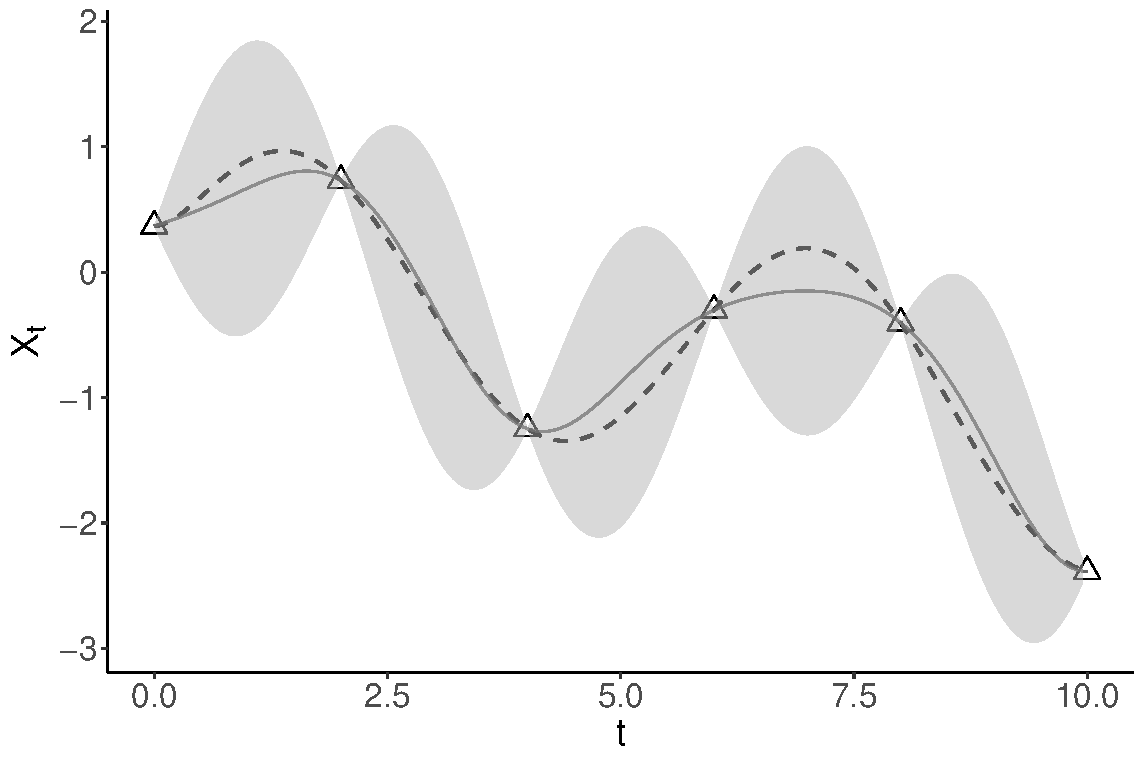
\includegraphics[scale=0.5]{GP1.pdf}
	\caption{Gaussian process regression used to estimate a function $f = X_t$ (shown in dotted grey lines). The prediction is based on the conditional mean of a noise-free GP with squared exponential function, which is shown in a line and was fitted based on 6 observations of $f$ (the triangle shapes). 95\% confidence bands computed using the conditional variance are also shown.}
	\label{fig:GP1}
\end{figure}



It is easy to extend this idea for cases in which, rather than having access to exact values of the function $f$, only estimates with some noise are available. This is the case, for example, when $f$ is simply impossible to evaluate, but can be reliably estimated via Monte Carlo methods---e.g. when $f$ is an expected loss over a high-dimensional parameter space. In these situations an additive noise term $\sigma^2$ is commonly added to the covariance function $\kappa$ for observations with the same covariates: $\kappa_{\sigma} (t, t') = \kappa(t, t') + \sigma^2 \, \indicator (t = t')$, where $\kappa$ is a regular noise-free covariance function. For any finite subset $T \subset \calT$, this can be represented as
\begin{equation*}
	K_{\sigma} (X_T, X_T) = K(X_T, X_T) + \sigma^2 \, I_{|T|},
\end{equation*}
so that
\begin{equation} \label{eq:GP_noise}
	X_T \equdist \calN \left( 0, \, K(T, T) + \sigma^2 \, I_{|T|} \right).
\end{equation}
The resulting conditional distribution for a new covariate value $t^{*}$ given $T$ is
\begin{equation*}
 \bbP [X_{t^{*}} \,| \, \sigma X_T ] \equdist \calN \left( K(t^{*}, T) \left( K(T, T) + \sigma^2 \, I_{|T|} \right)^{-1} X_T, \, \kappa(t^{*}, t^{*}) K(t^{*}, T) \left( K(T, T) + \sigma^2 \, I_{|T|} \right)^{-1} K(T, t^{*})  \right).
\end{equation*}



\subsection{Exchangeability of Gaussian processes}


Let $X = (X_t)_{t \in \calT} \sim \GP (0, \kappa)$. The process $X$ is said to be noise-free if Equation (\ref{eq:GP_noise_free}) holds and $\sigma$-noisy if Equation (\ref{eq:GP_noise}) holds for any finite subset $T \subset \calT$. We enforce the distinction because it has much influence on whether a process is exchangeable or not. Lastly, we also assume that $\kappa$ is given by Equation (\ref{eq:sq_exp_cov}), possibly with a modification to account for noisy observations if necessary, and that $\calT \subset \bbR$.



\begin{proposition} \label{prop:exchangeability}
	Let $X = (X_t)_{t \in \calT} \sim \GP (0, \kappa)$. Then $X$ is not exchangeable.
\end{proposition}

\textbf{Proof. \hspace{0.05cm}} Conceptually this is trivially true, and is due to the fact that the covariance function $\kappa$---which completely determines the process---is sensible to the distance between covariates. The order of the covariates matters, and so the sequence cannot be exchangeable. Formally, let $T = \{ t_1, t_2, t_3 \}$ with $t_2 = t_1 + 1, t_3 = t_1 + 2$ and $\pi$ be a permutation of $T$ such that $\pi(t_1) = t_2$,  $\pi(t_2) = t_1$, and $\pi(t_3) = t_3$. Then $X_T = \calN (0, K(T, T))$ and $X_{\pi T} = \calN(0, K(\pi T, \pi T))$---possibly with an additional term if the process is noisy. If $X$ were exchangeable, then $X_T \equdist X_{\pi T}$, and particularly $\kappa(t_1, t_3) = \kappa(t_2, t_3)$, which is clearly not the case because $\kappa(t_1, t_3) = e^{-1}$ but $\kappa(t_2, t_3) = e^{-1/2}$, regardless of whether the process is noisy or not.

\qed

\vskip 0.2cm

One may argue that this result is more due to the specific covariance function we chose rather than some underlying principle, but this is not so: the covariance function \textit{has} to be sensible to some notion of distance between covariates because we assume that close covariates will yield somewhat similar values of the function. The prediction of the process at $t^{*}$ includes information from all observations in $T$, but naturally those values in $T$ closer to $t^{*}$ will have a greater weight on the estimate $\bbE [X_{t^{*}} \, | \, \sigma X_T ]$. \\


The exchangeability requirement in Proposition \ref{prop:exchangeability} can be weakened to yield positive results, as we now show.

%but first we follow \cite{CampbellEtAl:2019:LocalExch} and introduce the following notation. Let $X = (X_t)_{t \in \calT}$ be a noisy Gaussian process with $\calT = \bbR$. If it is possible to obtain multiple observations at a single value, then it makes sense to modify $\calT$ by $\tilde{\calT} = \bbR \times \bbN$, where the first entry would denote the location of the observation and the second one the number of observation. So $\tilde{t} = (0.56, 2)$ would refer to the second observation at the value $t = 0.56$. In such a scenario we use both $\calT$ and $\tilde{\calT}$ interchangeably depending on the context; particularly when dealing with local exchangeability, using $\tilde{\calT}$ is more convenient. \\


\begin{proposition} \label{prop:GP_partial_exch}
	Let $X = (X_t)_{t \in \calT} \sim \GP (0, \kappa)$ be a $\sigma$-noisy Gaussian process. Then $X$ is partially exchangeable.
\end{proposition}

\textbf{Proof. \hspace{0.05cm}} The idea is to group the process into sequences with the same covariate value and prove that each of those is exchangeable. Formally, let $X_{t_0} = (X_{t_0, \, n})_{n=1}^{\infty}$ be the $t_0$-class of $X$ for each (distinct) $t_0 \in \calT$. Let $N = \{n_1, ..., n_r \}$ and $\pi$ a permutation of $N$. The key observation here is that $\kappa(t_0, t_0) = 1$, and so
\begin{equation} \label{eq:GP_partial_exchangeability}
	X_{t_0 \, N} \equdist \calN (0, (1+\sigma^2) I_r) \equdist X_{t_0 \, \pi N}.
\end{equation}
This proves that each $t_0$-class is exchangeable, and thus the whole process is partially exchangeable.

\qed

\vskip 0.2cm

A good question is whether a noise-free GP is partially exchangeable. We argue to the contrary, asserting---as in the previous section---that partial exchangeability is defined with replicates in mind. If a function can be precisely estimated (even if expensively so) at any given value $t$, it makes no sense to obtain replicates: there is no within-covariate variability. 
\\

%Indeed, if one attempts to replicate the previous proof then Equation (\ref{eq:GP_partial_exchangeability}) still holds, albeit with degenerate Normals that have zero variance. \\



In preparation for the main local-exchangeability results for GP regression, we state a sufficiency condition for determining local exchangeability of a sequence. For a proof, see \cite[][Proposition 3]{CampbellEtAl:2019:LocalExch}.

\begin{proposition} \label{prop:sufficient_local_exchangeability}
	Consider a process $(X_t)_{t \in \calT}$ and suppose there exists a $\sigma$-algebra $\calG$ such that, for any finite subset $T \subset \calT$ of covariates, the components of $X_T$ are conditionally independent given $\calG$. Let $G_t = \bbP [X_t \, | \, \calG ]$. Then $X$ is $f$-locally exchangeable if, for all pairs $t, t' \in \calT$,
	\begin{equation} \label{eq:sufficient_local_exchangeability}
		\bbE[d_{\mathrm{TV}} (G_t , G_{t'} ) ] \leq f(d(t, t')).
	\end{equation}
\end{proposition}

Now we assert that $\sigma$-noisy GPs are $f$-locally exchangeable, where $f$ is inversely proportional to the noise factor $\sigma$. 

\begin{proposition} \label{prop:GP_local_exchangeability}
	Let $f(x) = x / \pi \sigma$ and $X = (X_t)_{t \in \bbR} \sim \GP (0, \kappa)$ be a $\sigma$-noisy Gaussian process in $\bbR$, which we furthermore endow with the metric  $d(t, t') = |t-t'|$. Then $X$ is $f$-locally exchangeable.
\end{proposition}



\textbf{Proof. \hspace{0.05cm}} We prove that the requirements of Proposition \ref{prop:sufficient_local_exchangeability} are met. First observe that
\begin{equation*}
	\kappa(t, t') = \mathrm{exp} \left\{ -\frac{1}{2} |t - t'|^2 \right\} \geq 1 - \frac{1}{2} |t-t'|^2 = 1 - \frac{1}{2} d(t, t')^2,
\end{equation*}
which can be proved via the Taylor series expansion of $\mathrm{exp} \left\{ -\frac{1}{2} y^2 \right\}$. This can also be rewritten as
\begin{equation} \label{eq:kappa_bound}
	1 - \kappa(t, t') \leq \frac{1}{2} d(t, t')^2.
\end{equation}
Now let $T \subset \bbR$ be a finite subset of covariates of size $n$. Denoting $K(T, T) = K$, by Equation (\ref{eq:GP_noise}) we have that $X_T \equdist \calN (0, K + \sigma^2 I_n )$. Now let $Y_T \equdist \calN(0, K)$ and observe that
\begin{equation}
	\bbP [X_T \, | \, \sigma Y_T ] \equdist \calN(Y_T, \sigma^2 I_n).
\end{equation}
Thus, for every $t \in T$ the conditional distribution of $X_t$ given $Y_t$ is $G_t \equdist \calN (Y_t, \sigma^2)$. We need only prove that $\bbE[d_{\mathrm{TV}} (G_t , G_{t'} ) ] \leq f(d(t, t'))$. But, as per \cite[][p.~15]{CampbellEtAl:2019:LocalExch}, the total variation between two Normal distributions can be expressed in terms of the cumulative distribution function $\Phi$ of a standard Normal distribution, and so
\begin{align}
	d_{\mathrm{TV}} (G_t , G_{t'} )  &= d_{\mathrm{TV}} (\calN (Y_t, \sigma^2) , \calN (Y_{t'}, \sigma^2) )   \nonumber \\
		&= \Phi \left( \frac{|Y_t - Y_{t'} |}{2 \sigma} \right) - \Phi \left( -\frac{|Y_t - Y_{t'} |}{2 \sigma} \right) \nonumber \\
		&\leq \frac{|Y_t - Y_{t'} |/2\sigma + |Y_t - Y_{t'} |/2\sigma}{\sqrt{2\pi}} && \text{(by Lemma \ref{lemma:lipschitz})} \nonumber \\
		&= \frac{|Y_t - Y_{t'}|}{\sqrt{2 \pi \sigma^2}}. \label{eq:TV_GP}
\end{align}
Now, observe that $\kappa(t, t) = 1$ for all $t \in \bbR$, and so $Y_t, Y_{t'} \equdist \calN(0, 1)$ are Normal (and jointly Normal too by construction). Furthermore, $\mathrm{cov}(Y_t, Y_{t'}) = \kappa(t, t')$, and so by Lemma \ref{lemma:halfnormal}
\begin{equation*}
	\bbE |Y_t - Y_{t'}| = \sqrt{\frac{4}{\pi}(1 - \kappa(t, t'))}.
\end{equation*}
Substituting in Equation (\ref{eq:TV_GP}) we deduce
\begin{equation} \label{eq:TV_GP_2}
	\bbE [d_{\mathrm{TV}} (G_t , G_{t'} )] \leq \sqrt{\frac{2}{\pi^2 \sigma^2}(1 - \kappa(t, t'))}.
\end{equation}
Using $\kappa$'s lower bound (Equation \ref{eq:kappa_bound}) we finally get that, for all $t, t'$,
\begin{equation}
	\bbE [d_{\mathrm{TV}} (G_t , G_{t'} )] \leq \sqrt{\frac{1}{\pi^2 \sigma^2}d(t, t')^2} = \frac{d(t, t')}{\pi \sigma}.
\end{equation}
The result follows from Proposition \ref{prop:sufficient_local_exchangeability} with $f(x) = \frac{x}{\pi \sigma}$.

\qed


\vskip 0.25cm

It is not immediately clear from the proof whether this result holds for noise-free GPs. The argument essentially splits the variability in each observation into the variability within ($\sigma$) and between ($K$) covariates, and takes advantage of the fact that the within-covariate variability does not depend on the actual value of the covariate. But if no replicates are available, the argument no longer works and the function $f$ is not even defined, for we would have $\sigma = 0$. \\

On the other hand, recalling the definition of local exchangeability (Definition \ref{def:local_exchangeability}), it is intuitively clear that noise-free GPs should be locally exchangeable. It turns out that it is possible to modify the previous argument to get a positive result for noise-free GPs. We state the result, although the proof is left as an exercise.



\begin{proposition} \label{prop:GP_NF_local_exchangeable}
	Let $f(x) = (2/\pi) x$ and $X = (X_t)_{t \in \bbR} \sim \GP (0, \kappa)$ be a noise-free Gaussian process in $\bbR$, which we furthermore endow with the metric  $d(t, t') = |t-t'|$. Then $X$ is $f$-locally exchangeable.
\end{proposition}

\textbf{Proof. \hspace{0.05cm}} See Exercise \ref{ex:GP_NF_local_exchangeable}. \\



We now assert the corresponding result for regression exchangeability.


\begin{proposition} \label{prop:GP_reg_exch}
	Let $X = (X_t)_{t \in \calT} \sim \GP (0, \kappa)$ be a Gaussian process. Then $X$ is regression exchangeable.
\end{proposition}



\textbf{Proof. \hspace{0.05cm}} Let $T_1, T_2 \subset \calT$ be finite and first assume $X$ is noise-free.
\begin{enumerate}
	\item For Condition \ref{cond:reg_exch_1}, suppose $T_1 \subset T_2$.  We know $X_{T_2} \equdist \calN (0, K(T_2, T_2))$, and basic properties of the Normal distribution tell us that the distribution of $X_{T_1}$ is the same as that of $X_{T_2}$ but removing the coordinates in $T_2 \setminus T_1$.
	\item For Condition \ref{cond:reg_exch_2}, suppose $T_1 = T_2$. Because the process is noise-free, this means that $X_{T_1} = X_{T_2}$ exactly, and so $X_{T_1} \equdist X_{T_2}$.
\end{enumerate}
The case for $\sigma$-noisy GPs follows from simple modifications to the previous arguments. Namely, $X_{T_2} \equdist \calN( 0, K(T_2, T_2) + \sigma I)$ and the distribution of $X_{T_1}$ is again obtained by coordinate deletion for Condition \ref{cond:reg_exch_1}. For Condition \ref{cond:reg_exch_2} the only caveat is that $X_{T_1}$ and $X_{T_2}$ may contain different replicates, but they do so at the same covariates, and so both follow the same $\calN (0, K(T, T) + \sigma I)$ distribution, with common $T = T_1 = T_2$.

\qed






% ...

\vskip 2cm


% open questions section
% !TEX root = ../main.tex

% open questions section

\section{Discussion} \label{section:discussion}


The main question posed by this work was whether exchangeability could have any role in dependence modelling, and especially in Gaussian process regression. Proposition \ref{prop:exchangeability} implies that de Finetti's classical representation theorem cannot be used in such a setting. It is easy to conclude the same for other dependence modelling settings, such as regression analysis. 
\\


However, GP regression does satisfy more general notions of exchangeability: local and regression exchangeability for all GPs, and partial exchangeability for noisy GPs. It is clear that other dependence models also satisfy some of them. For example, the proof of Proposition \ref{prop:GP_reg_exch} can be easily adapted for linear regression analysis and ANOVA models. Furthermore, by Propositions \ref{prop:GP_partial_exch} and \ref{prop:GP_local_exchangeability} we know that any noisy GP can be represented as a conditional independence sequence as in Theorems \ref{thm:definetti_partial} and \ref{thm:de_finetti_local}, respectively. Proposition \ref{prop:GP_NF_local_exchangeable} guarantees such a representation for noise-free processes too. This is summarised in Table \ref{table:summary}.
\\






\begin{table}[h]
\centering
\begin{tabular}{l|cc|cc}
                & \multicolumn{2}{c|}{Noise-free}                                              & \multicolumn{2}{c}{Noisy}                                                     \\  
Exchangeability & \begin{tabular}[c]{@{}c@{}}Satisfies\\ definition\end{tabular} & \begin{tabular}[c]{@{}c@{}}Representation\\ theorem\end{tabular} & \begin{tabular}[c]{@{}c@{}}Satisfies\\ definition\end{tabular} & \begin{tabular}[c]{@{}c@{}}Representation \\ theorem\end{tabular} \\ \hline
Classical       & No        & No                                                               & No        & No                                                                \\
Partial         & No        & No                                                               & Yes       & Yes                                                               \\
Local           & Yes       & Yes                                                              & Yes       & Yes                                                               \\
Regression      & Yes       & No                                                               & Yes       & No                                                               
\end{tabular}
\caption{Summary of findings for GP regression and exchangeability. For each notion of exchangeability, does GP regression (either noise-free or noisy) satisfy the definition and, if so, are there any representation theorems available?}
\label{table:summary}
\end{table}




There seems to be a trade-off between adequacy and theoretical power in these notions of exchangeability: partial exchangeability is generally easy to verify and has a de Finetti-like representation theorem, but settings in which no replicates---and a countable number of them at that---are available are never going to exhibit partial exchangeability. Regression exchangeability is also easy to verify and, furthermore, satisfied by more general processes, but it lacks a representation theorem. Lastly, local exchangeability is a more powerful theoretical tool than both, but it is still unclear what processes exhibit this characteristic. It would appear that many do, but this remains to be proved. We expand these points in the research directions section below.




\subsection{Open questions and research directions}


From those exchangeability notions studied here, local exchangeability appears to be the most flexible: many real life processes naturally exhibit \textit{near} exchangeability. The fact that de Finetti's result proves robust to perturbations of exact exchangeability is remarkable. 
\\


However, as we hope to have made evident in this work, proving that a certain process is locally exchangeable is a complicated task at best---even with the sufficiency conditions of Proposition \ref{prop:sufficient_local_exchangeability}. \cite{CampbellEtAl:2019:LocalExch} prove that some popular Bayesian nonparametric models are locally exchangeable, but much work remains to be done in this respect. A first approach would be to simply prove, model by model, whether a certain process is locally echangeable or not, and under what conditions, until a sufficiently large repertoire of locally exchangeable processes is available. 
\\

Nonetheless, a more general result would be ideal, both from a theoretical and a practical point of view. It seems that the task of finding a suitable function $f$ is what tends to complicate matters, and so it would be desirable to obtain an existence-type theorem. That is, perhaps the question to be asked is not \textit{what} $f$ works, but under what conditions such an $f$ exists, which would then exhibit a process as locally exchangeable without having to manually compute $f$. We pursue this point a little bit further. \cite{CampbellEtAl:2019:LocalExch} show that $f$---specifically its rate of decay---plays a role in controling the smoothness of local exchangeability. Perhaps an ideal result would allow us to know not only if an $f$ that renders a process $f$-locally exchangeable exists, but also its rate of decay.
\\


Lastly, regression exchangeability is also easy to verify for any given sequence and would seem to be an ideal setting for most of dependence modelling---at the very least for regression analysis. It is however without a representation theorem, and thus determining if one exists would make it a much more valuable notion. In this spirit, we conjecture how such a result would look.
\\


Theorem \ref{thm:definetti_partial}---partial exchangeability representation theorem---essentially says that the classes of a partially exchangeable process exhibit conditional independence (although not i.i.d. behaviour, as in classical exchangeability). A result for regression exchangeability can be expected to capture the same idea, although instead of classes we would have samples with same covariate values. In other words, if a partially exchangeable sequence can be arranged by its exchangeable classes, a regression exchangeable one can be arranged by its samples. Hence, for such a process $(X_t)_{t \in \calT}$ we define, for every finite $T \subset \calT$,
\begin{equation*}
	\calE (T) = \{ T' \subset \calT \, : \, T' = T \}.
\end{equation*}
Observe that this specifies equivalence classes in the covariates: $T' \in \calE (T)$ if and only if $T \in \calE (T')$. Let $d$ be the number of such classes ($d$ may very well be $\infty$). We would expect this classes to be conditionally independent given some measure $\mu$ on $\calP^d$, where again $\calP$ is the set of probability measures in $(\calX, \calB)$. This leads us to the following conjecture.

\begin{conjecture} \label{conjecture:definetti_regression}
	The sequence $(X_t)_{t \in \calT}$ is regression exchangeable if and only if there exists a unique probability measure $\mu$ on $\calP^d$ such that, for all finite subsets $T_1, ..., T_d$ of each equivalence class, and for all $A_1, ..., A_d$ with $A_i \in \calB^{|T_i|}$,
	\begin{equation} \label{eq:definetti_regression_thm}
		\bbP \left\{ (X_{T_i}) \in A_i \, : \, i=1, ..., d  \right\} = \int_{\calP^d}  \prod_{i=1}^d F_i(A_i) \, \mu(dF_1, ..., dF_d).
	\end{equation}
\end{conjecture}

The right-hand side of Equation (\ref{eq:definetti_regression_thm}) may seem exactly the same as that in Theorem \ref{thm:definetti_partial}, but their meanings are inherently different: the former expresses exchangeability between samples, and the latter between classes. Proving Conjecture \ref{conjecture:definetti_regression}, or a suitable modification of it, may lead to a better understanding of the role of exchangeability in dependence modelling.





























%%%% appendix
\clearpage
\appendix

% exercises and problems
% !TEX root = ../main.tex

% Exercises section

\section{Exercises}


\begin{exercise}[Adapted from \cite{Kingman:1978}] \label{ex:n_symmetric}
	Let $X = (X_n)_{n=1}^{\infty}$ be an exchangeable sequence of random variables taking values in a measurable space $(\calX, \calF)$ with common expectation. A random variable $Y = g(X)$ is said to be $n$-\textit{symmetric} if it is bounded and invariant under permutations of its first $n$ components, that is, if
	\begin{equation} \label{eq:n_symmetric}
		g(X_1, X_2, ...) = g(X_{\pi(1)}, ..., X_{\pi(n)}, X_{n+1}, ...)
	\end{equation}
	for every permutation $\pi$ of $\bbN_n$. Define $\calF_n$ to be the smallest $\sigma$-algebra with respect to which all $n$-symmetric random variables are measurable. Let $f$ be an integrable numerical $\calF$-measurable function, that is, $\bbE |f(X_n)| < \infty$ for all $n$. Prove that $\frac{1}{n} \sum_{j=1}^n f(X_j)$ is a version of $\bbE[ f(X_1) \, | \, \calF_n ]$ for every $n$.
\end{exercise}

\textbf{Solution \ref{ex:n_symmetric}. \hspace{0.05cm}} Fix $n \in \bbN$. Because the components of $X$ have common expectation, clearly $\bbE[f(X_1)] = \bbE[f(X_j)]$ for every $1 \leq j \leq n$ and, moreover, $\bbE[ f(X_1) g(X) ] = \bbE[ f(X_j) g(X) ]$ for every $g \in \calF_n$. Thus,
\begin{equation*}
	\bbE \left[ \frac{1}{n} \sum_{j=1}^n f(X_j) g(X) \right] = \frac{1}{n} \sum_{j=1}^n \bbE[ f(X_j) g(X) ] = \frac{1}{n} \sum_{j=1}^n \bbE[ f(X_1) g(X) ] = \bbE[ f(X_1) g(X) ],
\end{equation*}
and so $\frac{1}{n} \sum_{j=1}^n f(X_j)$ satisfies the projection property. Furthermore, it is clearly $n$-symmetric as a function of $X$, and hence is in $\calF_n$, which completes the proof. \\
\qed

\vskip 0.25cm

Observe also that $\calF_{n+1} \subset \calF_n$: if a function is $n+1$-symmetric it is also $n$-symmetric. A reverse-martingale argument \cite[see Theorem B.124 (Lévy's theorem: part II) in][p.~650]{Schervish:1995} can be used to show that
\begin{equation} \label{eq:LLN_exch}
	\lim_{n \to \infty} \frac{1}{n} \sum_{j=1}^n f(X_j) = \bbE[ f(X_1) \, | \, \calF_{\infty}] \quad \mathrm{a.s.}, 
\end{equation}
where
\begin{equation*}
	\calF_{\infty} = \bigcap_{n=1}^{\infty} \calF_n.
\end{equation*}
Equation (\ref{eq:LLN_exch}) is a version of the Strong Law of Large Numbers for exchangeable sequences.

\vskip 0.75cm


\begin{exercise} \label{ex:GP_NF_local_exchangeable}
	Let $f(x) = (2/\pi) x$ and $X = (X_t)_{t \in \bbR} \sim \GP (0, \kappa)$ be a noise-free Gaussian process in $\bbR$, which we furthermore endow with the metric  $d(t, t') = |t-t'|$. Then $X$ is $f$-locally exchangeable. \\
	
	Hint: observe that $\kappa(t, t) = 1$.	For a finite subset $T \subset \bbR$, define $Y_T \equdist \calN ( 0, \tilde{K} )$, where $\tilde{K}$ is a matrix equal to $K(T, T)$ but with the diagonal elements divided by half.
\end{exercise}


\textbf{Solution \ref{ex:GP_NF_local_exchangeable}. \hspace{0.05cm}} Let $T \subset \bbR$ be a finite subset of size $n$ of the covariate space. We know that $X_T \equdist \calN (0, K)$, where $K = K(T,T)$. Furthermore, the diagonal of $K$ consists of 1's: $\kappa(t, t) = 1$ (see Equation (\ref{eq:sq_exp_cov}) with $\ell = 1$). Define $\tilde{K}$ to be a matrix equal to $K$ but with its diagonal elements divided by half:
\begin{equation*}
	\tilde{K}_{ij} = \begin{cases}
					  	\frac{1}{2}, & i=j, \\
					  	\kappa(t_i, t_j) & i \neq j.
					  \end{cases}
\end{equation*}
Now let $Y_T \equdist \calN(0, \tilde{K})$ and observe that $\bbP [ X_T \, | \, \sigma Y_T ] \equdist \calN \left( Y_T, \frac{1}{2} I_n \right)$. In other words, $X_T$ are conditionally independent given $Y_T$ because the latter captures the dependence structure in the sample. The argument that follows from here is identical to that of Proposition \ref{prop:GP_local_exchangeability}:
\begin{align*}
	d_{\mathrm{TV}} \left( \calN \left( Y_t, \frac{1}{2} \right) , \calN \left( Y_{t'}, \frac{1}{2} \right) \right) &= \Phi \left( |Y_t - Y_{t'} | \right) - \Phi \left( -|Y_t - Y_{t'} | \right) \\
		&\leq \sqrt{\frac{2}{\pi}} |Y_t - Y_{t'}|. && \text{(by Lemma \ref{lemma:lipschitz})}
\end{align*}
Now by Lemma \ref{lemma:halfnormal}
\begin{equation*}
	\bbE | Y_t - Y_{t'} | = \sqrt{\frac{4}{\pi}(1 - \kappa(t, t'))}
\end{equation*}
and so
\begin{equation*}
	\bbE \left[ d_{\mathrm{TV}} \left( \calN \left( Y_t, \frac{1}{2} \right) , \calN \left( Y_{t'}, \frac{1}{2} \right) \right) \right] \leq \sqrt{\frac{8}{\pi^2}(1 - \kappa(t, t'))} \leq \frac{2}{\pi} d(t, t'),
\end{equation*}
from where the result follows by Proposition \ref{prop:sufficient_local_exchangeability}.

\qed 



\vskip 2cm

% any other appendix sections
% !TEX root = ../main.tex

% additional technical results section

\section{Additional technical results}


\begin{lemma} \label{lemma:lipschitz}
	Let $\Phi$ and $\phi$ denote the \textit{cdf} and \textit{pdf} of a standard Normal distribution, respectively. Then, for $x_1 \leq x_2$,
	\begin{equation*}
		\Phi(x_2) - \Phi(x_1) \leq \frac{x_2 - x_1}{\sqrt{2 \pi}}.
	\end{equation*}
	In other words, $1/\sqrt{2 \pi}$ is a Lipschitz constant of $\Phi$.\footnote{Actually, it is \textit{the} Lipschitz constant of $\Phi$, although we only prove the weaker result here stated for the sake of brevity.}
\end{lemma}


\textbf{Proof. \hspace{0.05cm}} Recall that $\phi(x) \leq \phi(0) = 1 / \frac{1}{2\pi}$, from where trivially
\begin{equation*}
	\Phi(x_2) - \Phi(x_1) = \int_{x_1}^{x_2} du \, \phi(u) \leq \frac{1}{\sqrt{2 \pi}} \int_{x_1}^{x_2} du = \frac{x_2 - x_1}{\sqrt{2 \pi}}.
\end{equation*}
\qed



\begin{lemma} \label{lemma:halfnormal}
	Let $X_1 \sim \calN(0, \sigma_1^2)$ and $X_2 \sim \calN(0, \sigma_2^2)$ be Normal random variables with covariance $\sigma_{12}$. Then $\bbE |X_1 - X_2| = \sqrt{\frac{2}{\pi} (\sigma_1^2 + \sigma_2^2 - 2\sigma_{12})}$.
\end{lemma}

\textbf{Proof. \hspace{0.05cm}} We have that $X_1 - X_2 \sim \calN(0, \sigma_1^2 + \sigma_2^2 - 2\sigma_{12})$, and so $W := |X_1 - X_2| \sim \mathrm{HN} (\sqrt{\sigma_1^2 + \sigma_2^2 - 2\sigma_{12}})$, where HF refers to the Half-Normal distribution. Indeed, it is well known that if $U \sim \mathrm{HN} (\xi)$ then $\bbE[U] = \sqrt{2 / \pi} \xi$, from where result follows.

\qed





% bibliography
%\nocite{*}
\clearpage
\printbibliography

\end{document}